\documentclass{article} % For LaTeX2e
\usepackage{latex_template,times}
\usepackage{hyperref}
\usepackage{url}
\usepackage{euler}
\usepackage{natbib}
\usepackage{amsmath}
\usepackage{prettyref}
\usepackage[]{hyperref}
\usepackage{mathtools}
\usepackage{csvsimple}
\usepackage{booktabs}
\DeclarePairedDelimiter{\norm}{\lVert}{\rVert}
% in dvi it only seems to use urlcolor !!!!
\hypersetup{colorlinks,linkcolor=blue,citecolor=blue,pagecolor=blue,%
            urlcolor=magenta,filecolor=magenta,breaklinks,%
            dvips,bookmarks,bookmarksopen}
%\documentstyle[nips14submit_09,times,art10]{article} % For LaTeX 2.09

%\author{Chen C che5002 480458339, Yutong Cao ycao5602 470347494,***}
\title{Assignment 2}

\newcommand{\fix}{\marginpar{FIX}}
\newcommand{\new}{\marginpar{NEW}}
\newcommand{\svm}{\textsc{svm}}

\nipsfinalcopy % Uncomment for camera-ready version

\begin{document}

\author{%
 \begin{tabular}{rl}
  Tutors: & Zhuozhuo Tu, Liu Liu\\ \\
Group members: & Chen Chen (cche5002) 480458339, \\
& Yutong Cao (ycao5602) 470347494,\\
& Yixiong Fang ***
\end{tabular}
}

\maketitle



\begin{abstract}
This report documents our modifications to the soft-margin support vector machine to improve its performance against class-dependent classification noise where the flip rates are $0.2$ and $0.4$.
\end{abstract}
\section{Introduction}
This report documents our modifications to the soft-margin support vector machine~(\svm) to improve its performance against class-dependent classification noise (\textsc{ccn}).

The capability of learning with label noise is crucial for training machine learning models. According to the law of large numbers \citep{hardle2007applied}, the empirical risk converges to the expected risk only if sample size is large. However,  classification labels in large data set can be easily corrupted. For example, images  are sometimes labelled manually by employing casual staff with minimal training. In this case, training a classification models using these images requires special treatment that accounts for noisy labels. Section~\ref{method} proposes three such treatments based on \svm\ to increase the accuracy with presence of \textsc{ccn}.

%maybe move to related work
%Usually there is a trade-off between the data complexity and the data quality ({\color{red} reference!}). Weakly supervised learning methods are introduced to handle this kind of problems ({\color{red} reference!}). For example, positive and unlabelled learning and semi-supervised learning are designed to trade data complexity for data quality. They both make use of a small set of correct data to train a model. Also there is learning with noisy labels, on the contrary, trades data quality for data complexity. It learns a model with a large amount of noisy data. In this assignment, we only focused on the latter.

 %For both data sets, the flip rates are given. 
Section~\ref{1st} proposed a learning method by deriving a new loss function using expectation maximisation \citep[p.423]{Bishop:2006:PRM:1162264}. This method models the label noise using a Bernoulli distribution, and includes the label noise information into the loss function of \svm. This method is first studied by \citet{pmlr-v20-biggio11} for random classification noise (\textsc{rcn}), and we extended it to \textsc{ccn}. 

Section~\ref{2nd} introduces a heuristic approach based on the work of \citet{Wu03probabilityestimates}. This method follows the heuristic observation that the predicted probability of a sample point with wrong label is usually close to 0.5. In this case, our model is not capable of suggesting a prediction with confidence. We then exclude the potential noisy data points and train the model again with the remaining data which seems to be cleaner. 

Section~\ref{3rd} implements importance reweighting proposed by \citet{liu2016classification}. This method uses a reweighting coefficient to reweight the loss function for each sample point. We fit \svm s with the given noisy data. We then implement cross-validation of \svm\ models to predict the probabilities of classifying each sample, and then use these probabilities to calculate the weightings.

To fairly compare these three approaches of attacking noisy data, all of the three methods implement the same base classification algorithm---\svm. We use \svm\ because it is proved to has a strong generalisation ability \citep{NIPS2012_4500,Seeger:2003:PGE:944919.944929,Cortes1995}, and usually gives high classification accuracy when turned properly \citep{Fernandez-Delgado:2014:WNH:2627435.2697065}. 
%As a result,  it is not considered to be robust to label noise ({\color{red} gives reference})

Section~\ref{result} applies the three methods proposed in Section~\ref{method} to two sets of noisy data with binary labels, both containing $10,000$ images. The first data set is a subset of the fashion-\textsc{mnist} database and the second data set is from the \textsc{cifer} database. For each data set, Section~\ref{result} also compares the simulation results, including accuracy and running times, from the three methods. In addition, we estimate the flip rate using the method proposed by \citet{liu2016classification}. 
%We did not use the estimated values in our classification experiments as the true rates are provided. 
Section~\ref{result} also compares our estimation with the true values.

\section{Related work}
Many recent literature discusses the topic of learning with label noise. One popular approach is to use classification algorithms that are proved to be robust to label noise. \citet{frenay2014classification} reported their findings that $0-1$ loss and least-squares loss are robust loss functions to uniform label noise. %compared $179$ classifiers from $17$ families on $121$ data sets. 
They also found the method of bagging is robust against label noise. Bagging detect the contaminated samples by estimating the variability of its base classifier when including and excluding them. %We chose not to use the robust loss functions as the corresponding classification models may not produce satisfying classification accuracy as \textsc{svm}. 
%But we used a bagging-like technique by sampling multiple times and averaging the predicted probabilities to generate better and more stable predictions. 
\citet{frenay2014classification} also discussed filtering methods for learning with label noise. These methods remove mislabelled data before training a final model. Our second model follows this idea by excluding data points with vague predictions. Instead of removing the contaminated candidates directly, \citet{yang2018adasampling} proposed a filter-like method that estimating the probability of mislabelling for each sample. 

These approaches mentioned above do not require noise rates. Although this makes the approaches general, the methods may not be able to handle highly contaminated data set, especially when the noise rates are given. \citet{pmlr-v20-biggio11} applies expectation maximisation method to fit data with \textsc{rcn}. This method reformulates the loss function to include noise rate information. The label noise is not usually observed. They use the expected value as an estimation of unobserved labels contaminated by noise. Section~\ref{1st} extends his method to solve problems with \textsc{ccn}. The idea behind this method is straightforward and intuitive, but  simulation results in Section~\ref{result} finds it is less accurate than the method of importance reweighting proposed by \citet{liu2016classification}. \citet{liu2016classification} assigned a weight to each sample according to its probability of being contaminated. These probabilities are estimated from a pre-train model. They also provided an efficient method for estimating the noise rate. However, the need of fitting the model twice makes the method of reweighting slow.

\section{Method}\label{method}
We use \textsc{svm} with Gaussian kernel as the base classification method for this task because of its generalisation ability.

\textsc{svm} with Gaussian kernel was first published by \citet{Boser:1992:TAO:130385.130401}. \citet{Cortes1995} proposed an improvement on the original \textsc{svm} with soft-margin  to  avoid over-fitting problem. The \textsc{svm} is to minimise the Hinge loss function
\begin{equation*}
\left[{\frac {1}{n}}\sum _{i=1}^{n}\max \left(0,1-y_{i}(w\cdot x_{i}-b)\right)\right]+\lambda \lVert w\rVert ^{2}.   
\end{equation*}
Here, $w$ is the weighting factor, $b$ is a constant. We classify the $i$th image into category~$1$ or~$-1$ when $w\cdot x_{i}-b\geq1$ or $w\cdot x_{i}-b\leq-1$, respectively. This loss function not only penalises points that misclassified, but also points that are closed to the dividing hyperplane, with a regularisation term~$\lambda \lVert w\rVert ^{2}$. \citet{Fernandez-Delgado:2014:WNH:2627435.2697065} suggested \svm\ is very likely to be one of the most powerful classifiers, by comparing 179 classification algorithms over 121 large data sets. The distances between data points and the dividing hyperplane gives an intuitive estimate of the generalisation ability of the trained \svm\ model \citep{hastie01statisticallearning}. 

we use \svm\ as our classification method as of its strong generalisation ability. In this image classification assignment, we do not observe the true labels~$y_i$. This section proposes three different approaches to modify ordinary \svm\ to attack label noise problem. However, we do not have access to a test data set with true labels~$(x_i,y_i)$ to verify the generalisation ability of our three different models, which are all trained by noisy data~$(x_i,S_i)$. Using \svm , the gap between hyperplane and the training data set provides a natural and `free' metric of its generalisation ability  \citep{hastie01statisticallearning}, and hence use of test data set is not mandatory. Using this geometry factor as well as probably approximately correct learning framework,  \citet{NIPS2012_4500} proved that the  \svm\ models have strong generalisation ability. Further,  \citep{Cortes1995,Seeger:2003:PGE:944919.944929} also shows the strong generalisation ability from different perspectives.

\subsection{Preprocess}
\texttt{StandardScaler} from \texttt{sklearn} was used. Each image is rescaled to have mean zero and standard deviation one. By doing this, we removed the brightness difference among different images. This process is called photometric normalisation. \citet{jonsson2002support} suggested that this may improve the performance of Gaussian kernel SVM as Gaussian kernel is a radius based kernel and hence it performs well when images are on the same scale. For the \textsc{cifer} dataset, we used principle component analysis (\textsc{pca}) for dimension reduction. We did not run \textsc{pca} on the fashion-mnist data because the dimension is reasonable.

\subsection{The original data set is balanced} \label{sec:1}
The assignment instruction states the probabilities~$P(S=1|Y=0)=0.2$ and $P(S=0|Y=1)=0.4$. From the data, we observed that $40\%$ of contaminated labels~$S$ (i.e. $P(S=1)$) is $1$. As a result
\begin{eqnarray*}
P(S=1)&=&P(S=1|Y=1)P(Y=1)+P(S=1|Y=0)P(Y=0)\\
     &=&\left[1-P(S=0|Y=1)\right]P(Y=1)+P(S=1|Y=0)P(Y=0)\\
     &=&0.6P(Y=1)+0.2\left[1-P(Y=1)\right]=0.4, \nonumber
\end{eqnarray*}
which implies $P(Y=1)=P(Y=0)=0.5$ and the original classification problem is balanced.In addition, define the Bernoulli random variable~$\epsilon(S)$ with the means $E(\mu(\epsilon)(S=0))=P(Y=1|S=0)=0.5\times0.4/0.6=1/3$ and $E(\epsilon(S=1))=P(Y=0|S=1)=0.5*0.2/0.4=0.25$. This random variable~$\epsilon$ describe the unobserved random label noise. Hence the expectation is
\begin{equation}
    E\epsilon(S)=P(Y=0|S=1)P(S=1)+P(Y=1|S=0)P(S=0)=0.25\times 0.4+1/3\times0.6=0.3.\label{eq:exp}
\end{equation}
\subsection{Method 1: Modified support vector machine}\label{1st}
This section extends the expectation maximisation algorithm proposed by \citet{pmlr-v20-biggio11} to modify \svm for labels noises. This section describes the mathematical justification for our modification.
%---the given label noise where flip rates~$P(S=1|Y=0)=0.2$ and~$P(S=0|Y=1)=0.4$ seems to be marginally different to a random label noise with flip rate~$P(S=1|Y=0)=P(S=0|Y=1)=0.3$ for \textsc{svm}.
\subsubsection{Expectation maximisation}
The original algorithm proposed by \citet{pmlr-v20-biggio11} was proposed to study classification problems with label noise where the flip rate $\rho_+=\rho_-$ and we extend it to manage the case dependent label noise where the flip rates $\rho_+\neq\rho_-$.

Recall the dual problem of an \textsc{svm} is to maximise
\begin{equation}
   f(c_{1}\ldots c_{n})=\sum _{i=1}^{n}c_{i}-{\frac {1}{2}}\sum _{i=1}^{n}\sum _{j=1}^{n}y_{i}c_{i}k(x_{i},x_{j})y_{j}c_{j}, \label{eq:dual}
\end{equation}
\begin{math}
{\text{subject to }}\sum _{i=1}^{n}c_{i}y_{i}=0,\,{\text{and }}0\leq c_{i}\leq {\frac {1}{2n\lambda }}\;{\text{for all }}i. 
\end{math} 
Here $y_i$ and $x_i$ are the labels and features of the $i$th image, $c_i$ is the $i$th Lagrangian multiplier, $k(x_i,x_j)$ is the Gaussian kernel product of $x_i$ and $x_j$ whose corresponding kernel is
\begin{equation*}
\exp(-\gamma\norm{x_i-x_j}).
\end{equation*}
Substitute label noise~$y_i=S_i(1-2\epsilon(S_i))$ into objective function~\eqref{eq:dual}
\begin{equation}
   f(c_{1}\ldots c_{n})=\sum _{i=1}^{n}c_{i}-{\frac {1}{2}}\sum _{i=1}^{n}\sum _{j=1}^{n}S_{i}c_{i}k(x_{i},x_{j})S_{j}c_{j}(1-2\epsilon(S_i))(1-2\epsilon(S_j)), \label{eq:dual2}
\end{equation}
When $i=j$, the expectation~$E(1-2\epsilon(S_i))(1-2\epsilon(S_j))=1-4E\epsilon(S_j)+4E\epsilon(S_j^2)=1$. When $i\neq j$, the expectation~$E(1-2\epsilon(S_i))(1-2\epsilon(S_j))=(1-2E\epsilon(S_i))(1-2E\epsilon(S_j))=1-\mu$ where parameter~$\mu:=0.84$, by substituting expectations~\eqref{eq:exp} from Section~\ref{sec:1}. 

Define kernel correction matrix~$M$ with the $(i,j)$-th entry being $m_{ij}$.The diagonal entries~$m_{ii}=1 $, and the off diagonal entries~$m_{ij}=1-\mu=0.16$ when indexes~$i\neq j$. Using the technique of Expectation maximisation, 
\begin{equation}
   Ef(c_{1}\ldots c_{n})=\sum _{i=1}^{n}c_{i}-{\frac {1}{2}}\sum _{i=1}^{n}\sum _{j=1}^{n}S_{i}c_{i}k(x_{i},x_{j})S_{j}c_{j}m_{ij}, \label{eq:dual3}
\end{equation}
The only difference between our modified \textsc{svm} and ordinary \textsc{svm} is to replace the kernel matrix~$K$ with our new proposed matrix~$Q:=K\circ M$.

\subsubsection{Tuning}
Define data vector~$\vec{x}:=(x_1,x_2,\ldots , x_n)$. The Kernel parameter for Gaussian Kernel~$\gamma$ is chosen to maximise the Variance of Kernel matrix~$K(\vec{x},\vec{x})$. The regularisation parameter is chosen to be one as the model seems to be insensitive to the regularisation parameter.

%\subsubsection{Additional regularisation}


%This soft-margin \textsc{svm} is sub-optimal for our problem. We have a large set of data ($10,000$) comparing with the number of features ($784$). Hence, we build a modified \textsc{svm} that aims to minimise the following Hinge loss
%\begin{equation}
%\left[{\frac {1}{n}}\sum _{i=1}^{n}\max \left(0,10-y_{i}(w\cdot x_{i}-b)\right)\right]+\lambda \lVert %w\rVert ^{2}.   \label{eq:pri}
%\end{equation}
%The modified constant~$10$ requires the predictor~$w\cdot x_{i}-b$ to be as extreme as possible, i.e., it penalises wrongly classified samples. Moreover, it even penalises correctly classified samples with small gaps between data points and the dividing hyper-plane being small. 
%Define $\zeta _{i}:=\max \left(0,10-y_{i}(w\cdot x_{i}-b)\right)$. The prime problem of Hinge loss~\eqref{eq:pri} becomes a minimisation of
%\begin{equation}
%{\frac {1}{n}}\sum _{i=1}^{n}\zeta _{i}+\lambda \|w\|^{2}
%{\text{ subject to }}y_{i}(w\cdot x_{i}-b)\geq 10-\zeta _{i}\,{\text{ and }}\,\zeta _{i}\geq 0,\,{\text{for all }}i. \label{eq:pri2}
%\end{equation} 
%The modification is inspired by observing that the regularisation parameter~$\lambda$ has a negligible impact on the classification results for this problem. Hence we have more than enough data to train this complex model without over fitting.

%The modified \textsc{svm} aims to make the algorithm more robust to label noise, even though it may enlarge the generalisation error. Nevertheless, the large data set will assure us the generalisation error is within a reasonable magnitude.
%The parameters~$c_i$ are Lagrangian multipliers that enforcing the condition~$y_{i}(w\cdot x_{i}-b)\geq 10-\zeta _{i}$ in prime problem~\eqref{eq:pri2}.

%With this modification, the dual problem~\eqref{eq:dual3} of the loss function~\eqref{eq:pri} becomes
%\begin{equation*}
%   Ef(c_{1}\ldots c_{n})=10\sum _{i=1}^{n}c_{i}-{\frac {1}{2}}\sum _{i=1}^{n}\sum %_{j=1}^{n}S_{i}c_{i}k(x_{i},x_{j})S_{j}c_{j}m_{ij}. \label{eq:dual3}
%\end{equation*}
%From the dual prospective, we are weakening the contributions of the contaminated labels~$S_i$, hence making the algorithm more robust.



This method gives us an accuracy of $94.6\%$ on the testing data.

\subsection{Method 2: heuristic approach}\label{2nd}
Method 2 still implement \textsc{svm}. We chose \textsc{svm} because classification algorithms with Hinge loss, including \textsc{svm}, is robust against random classification label noise. Our label noise is class dependent. However, experiment shows that \textsc{svm} is still robust against it.
%\subsubsection{Hinge loss is robust against label noise}

\subsubsection{Select samples}
Ordinary \textsc{svm} only gives a classification without revealing a probability that indicates the confidence of classification. \citet{Wu03probabilityestimates} proposed a five-fold cross-validation method to calculate the classification probabilities~$P(Y=1|X_i)$ for \textsc{svm}. 
Using this method, we calculated the probability~$P(Y=1|X_i)$ with label noise by an \textsc{svm} with Gaussian kernel. We have $10,000$ samples. We only use those with largest and smallest $P(Y=1|X_i)$ (first $1/3$ and last $1/3$), because intuitively the contaminated samples are more likely to have a probability~$P(Y=1|X_i)$ close to $0.5$ and the error rate $P(\epsilon=1)=0.3$. A $3\%$ margin was left because classification errors must exist.
\subsubsection{Label correction}
We relabel the $1/3$ of the samples with highest fitted probability~$P(Y=1|X_i)$ as $1$ and the $1/3$ samples with the smallest fitted probability~$P(Y=1|X_i)$ as $-1$. This step is important because section~\ref{sec:1} shows that the original data set is balanced ($P(Y=1)=P(Y=0)=0.5$). 

Training our \textsc{svm} with Gaussian Kernel again with this subset of relabeled data gives our second model.

This method gives us an accuracy of $95.0\%$ on the testing data.
%\subsubsection{Hinge loss if robust against label noise}
\subsection{Method 3: Reweighting} \label{3rd}
Please copy some formulae to here from tut11.

\section{Result}\label{result}
\begin{table}
\centering
    \scalebox{0.9}{
	\begin{tabular}{lllll}
\toprule
Data & Null Hypothesis ($H_0$) & $D$ & P-value & Reject $H_0$\\
\midrule
 & Relabelling algorithm is no more accurate than expectation maximisation.  & 0.625 & 0.0019 & Reject\\
 
 \textsc{mnist} & Expectation maximisation algorithm is as accurate as Reweighting. & 0.3125 & 0.4154 & Fail to reject\\
 
  & Reweighting algorithm is as accurate as relabelling. & 0.3125 & 0.4154 & Fail to reject\\
\bottomrule
   & Expectation maximisation algorithm is no more accurate than relabelling. & 0.5 & 0.0183 & Reject\\

 \textsc{cifar}  & Reweighting algorithm is no more accurate than expectation maximisation. & 0.6875 & 0.0005 & Reject\\

  & Reweighting algorithm is no more accurate than relabelling.  & 0.6875 & 0.0005 & Reject\\
\hline 
\end{tabular} }
	\caption{Hypothesis test}
	\label{tab:HypothesisTest}
\end{table}

\begin{table}
	\caption{Mean sd}
	\label{tab:Meansd}
% Please add the following required packages to your document preamble:
% \usepackage{booktabs}
\centering
\begin{tabular}{@{}lll@{}}
\toprule
Mean  & Standard deviation & Confidence interval \\ \midrule
0.938 & 0.003              & (0.936,0.939)       \\
0.942 & 0.003              & (0.941,0.944)       \\
0.94  & 0.003              & (0.939,0.942)       \\
0.835 & 0.004              & (0.833.0.837)       \\
0.832 & 0.008              & (0.829,0.836)       \\
0.844 & 0.005              & (0.841,0.846)       \\ \bottomrule
\end{tabular}

\end{table}



\begin{figure}    
	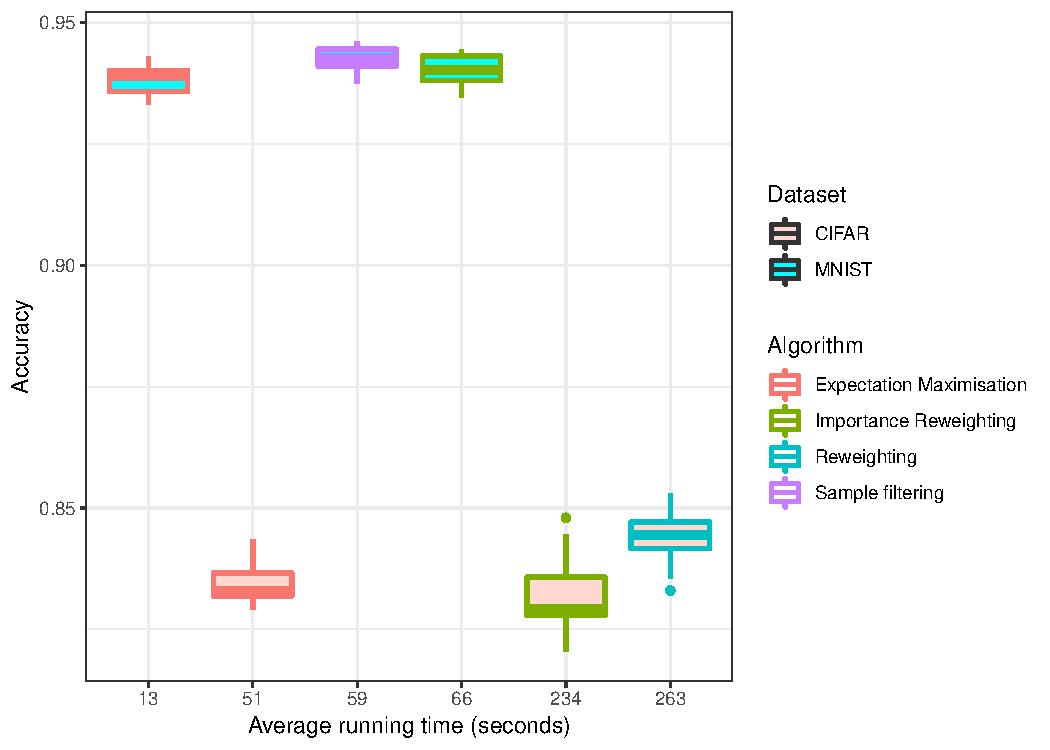
\includegraphics[scale=0.9]{boxplot.pdf}
	\caption{Boxplot}
	\label{fig:Boxplot}
\end{figure}

\begin{figure}    
	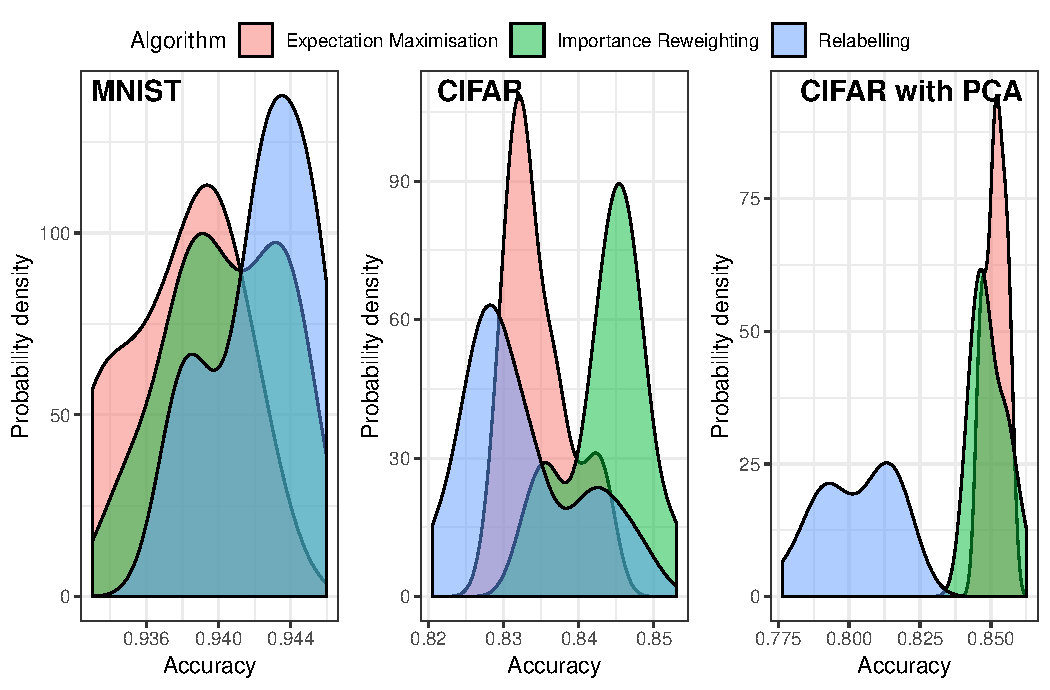
\includegraphics[scale=0.9]{histo.pdf}
	\caption{Density function from kernel smoothing}
	\label{fig:Density function from kernel smoothing}
\end{figure}

scatter plot of time vs. accuracy
histogram of accuracy
mean, sd table

Please pay special attention to the instructions in section \ref{others}
regarding figures, tables, acknowledgments, and references.

\section{Conclusion}
\label{headings}



\bibliographystyle{unsrtnat}
\bibliography{reference}



\end{document}
